\documentclass[11pt]{article}
\usepackage{mathblatt}
% gesetzt von werkzeuge/setzer.py (Sorte selbst) aus dem Lernweg FEU
% und den Bankzeilen; Muster bau/proben/2026-10-09/hypotenuse-muster.
\usepackage{enumitem}
\usepackage{adjustbox,varwidth}
\newgeometry{a4paper,margin=18mm,top=15mm,bottom=20mm,footskip=9mm}
\pagestyle{fancy}\fancyhf{}\renewcommand{\headrulewidth}{0pt}
\fancyfoot[L]{\footnotesize\color{mbgrau}FEU \textperiodcentered{} Quader und Würfel}
\fancyfoot[R]{\footnotesize\color{mbgrau}\thepage}
\setlength{\parskip}{3pt}
\renewcommand{\kreuz}[1]{\mbox{$\square$\ #1}\quad}
\newcommand{\kreuzl}[1]{\par\hangindent1.4em\hangafter1\noindent$\square$\ #1}
\newcommand{\aufg}[3]{\par\noindent\makebox[0pt][r]{#3}\begin{minipage}[t]{\linewidth}#1\end{minipage}\par}
\newcommand{\aufgg}[4]{\par\noindent\makebox[0pt][r]{#4}\begin{minipage}[t]{0.6\linewidth}\vspace{0pt}#1\end{minipage}\hfill
  \begin{minipage}[t]{0.37\linewidth}\vspace{0pt}\centering #2\end{minipage}\par}
\newcommand{\nr}[1]{\makebox[7mm][l]{\textbf{#1}}}
\newcommand{\lsg}[3]{\par\noindent\begin{minipage}[t]{9mm}\textbf{#1}\end{minipage}%
  \begin{minipage}[t]{52mm}\raggedright\bfseries\boldmath #2\end{minipage}\hspace{3mm}%
  \begin{minipage}[t]{\dimexpr\linewidth-64mm\relax}\raggedright\small #3\end{minipage}\par\vspace{4pt}}
\newlength{\kr}
\makeatletter
\newcommand{\karomerk}[2]{\protected@write\@auxout{}{\string\karoseite{#1}{#2}{\thepage}}}
\newcommand{\karoseite}[3]{\expandafter\xdef\csname karo@#1@#2\endcsname{#3}}
\newcommand{\karohinweis}[3]{\karomerk{h}{#1}\ifcsname karo@k@#1\endcsname
  \ifnum\csname karo@k@#1\endcsname=0\csname karo@h@#1\endcsname\relax#2\else#3\fi
  \else#3\fi}
\makeatother
\begin{document}

\noindent{\LARGE\bfseries Quader und Würfel}\par\smallskip
\noindent{\small\color{mbgrau}Selbstlernheft Klasse 6 \textperiodcentered{} mit Lösungsheft \textperiodcentered{} Kennung FEU}\par\medskip
\noindent\textbf{So nutzt du das Heft:} Lies im Abschnitt das Beispiel. Rechne dann die Aufgaben der Reihe nach und vergleiche jede sofort mit dem Lösungsheft. Kreuze „kann ich“ an, wenn du die letzte Aufgabe (\emph{Ziel}) allein schaffst.\par
\noindent Mehr Aufgaben zu einem Abschnitt: Kennung deinem Nachhilfelehrer schicken (z.\,B. „FEU mehr B“).\par\medskip
{\arrayrulecolor{mbgrau}\renewcommand{\arraystretch}{1.3}
\noindent\begin{tabular}{|>{\bfseries}p{10mm}|p{112mm}|>{\raggedleft\arraybackslash}p{10mm}|>{\centering\arraybackslash}p{14mm}|}\hline
\rowcolor{black!8} & \textbf{Abschnitt} & \textbf{Seite} & \textbf{kann ich}\\\hline
A & Volumen von Quader und Würfel & \pageref{s:A} & $\square$\\\hline
B & Oberfläche & \pageref{s:B} & $\square$\\\hline
C & Liter und Kubikzentimeter & \pageref{s:C} & $\square$\\\hline
D & Höhe aus dem Volumen & \pageref{s:D} & $\square$\\\hline
T & Probetest & \pageref{s:T} & $\square$\\\hline
\end{tabular}}\par\bigskip

\begin{tcolorbox}[colback=mbkasten,colframe=mbgrau,boxrule=0.5pt,arc=1mm,left=3mm,right=3mm,top=2mm,bottom=2mm,title={\bfseries Formel auf einen Blick},coltitle=black,colbacktitle=black!10]
{\Large Quader: $V = a \cdot b \cdot c$ \qquad $O = 2 \cdot a \cdot b + 2 \cdot a \cdot c + 2 \cdot b \cdot c$\par Würfel: $V = a \cdot a \cdot a$ \qquad $O = 6 \cdot a \cdot a$\par $1$ Liter $= 1$\,dm³ $= 1\,000$\,cm³}\par\medskip
In Worten: Volumen ist, was hineinpasst (cm³, Liter); Oberfläche ist die Hülle (cm²).\par\medskip
\end{tcolorbox}
\medskip\noindent\textbf{Typische Fehler – so nicht}\par\smallskip
\noindent\nr{$\times$}Volumen und Oberfläche vertauscht. Erst fragen: Inhalt oder Hülle?\par
\noindent\nr{$\times$}Beim Würfel nur $a \cdot a$ gerechnet. Das ist eine Fläche, nicht das Volumen.\par
\noindent\nr{$\times$}cm³ durch $100$ statt durch $1\,000$ geteilt, um Liter zu bekommen.\par
\clearpage\label{s:A}\noindent\colorbox{black!12}{\makebox[10mm]{\Large\bfseries\strut A}}\hspace{3mm}{\Large\bfseries Volumen von Quader und Würfel}\par\smallskip
\noindent Das \textbf{Volumen} sagt, wie viel in einen Körper hineinpasst: wie viele Würfel mit $1$\,cm Kantenlänge (je $1$\,cm³). Beim Quader rechnest du Länge mal Breite mal Höhe.\par\medskip
\noindent\textbf{Formel}\par\nopagebreak\noindent\hspace*{4mm}\begin{minipage}{\dimexpr\linewidth-4mm\relax}$V = a \cdot b \cdot c$ \qquad Würfel: $V = a \cdot a \cdot a$\end{minipage}\par\medskip
\noindent\textbf{Beispiel}\quad Eine Schachtel ist $5$\,cm lang, $3$\,cm breit und $4$\,cm hoch. Wie viele Zentimeterwürfel passen hinein? Wie groß ist ihr Volumen?\par\smallskip
\noindent\begin{minipage}[t]{0.6\linewidth}\vspace{0pt}\par\noindent\hangindent6mm\hangafter1\makebox[6mm][l]{\textbf{1}}Unten liegt eine Schicht: Länge mal Breite, $5 \cdot 3 = 15$ Würfel.\par\smallskip\par\noindent\hangindent6mm\hangafter1\makebox[6mm][l]{\textbf{2}}Die Schachtel ist $4$\,cm hoch, also $4$ Schichten: $15 \cdot 4 = 60$ Würfel.\par\smallskip\par\noindent\hangindent6mm\hangafter1\makebox[6mm][l]{\textbf{3}}Jeder Würfel ist $1$\,cm³. Volumen $V = 5 \cdot 3 \cdot 4 = 60$\,cm³. Misst du in dm, heißt die Einheit dm³.\par\smallskip\par\noindent\hangindent6mm\hangafter1\makebox[6mm][l]{\textbf{4}}Beim Würfel sind alle Kanten gleich. Kante $5$\,cm: $V = 5 \cdot 5 \cdot 5 = 125$\,cm³ (nicht $5 \cdot 5$).\par\smallskip\end{minipage}\hfill
\begin{minipage}[t]{0.37\linewidth}\vspace{0pt}\centering 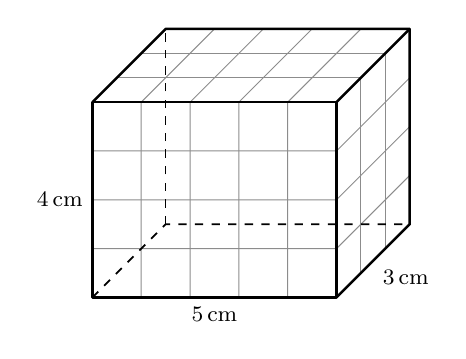
\begin{tikzpicture}[scale=0.62,font=\footnotesize,line join=round]\draw[black!45,line width=0.35pt] (1,0) -- (1,4) -- (2.5,5.5);\draw[black!45,line width=0.35pt] (2,0) -- (2,4) -- (3.5,5.5);\draw[black!45,line width=0.35pt] (3,0) -- (3,4) -- (4.5,5.5);\draw[black!45,line width=0.35pt] (4,0) -- (4,4) -- (5.5,5.5);\draw[black!45,line width=0.35pt] (0,1) -- (5,1) -- (6.5,2.5);\draw[black!45,line width=0.35pt] (0,2) -- (5,2) -- (6.5,3.5);\draw[black!45,line width=0.35pt] (0,3) -- (5,3) -- (6.5,4.5);\draw[black!45,line width=0.35pt] (0.5,4.5) -- (5.5,4.5) -- (5.5,0.5);\draw[black!45,line width=0.35pt] (1,5) -- (6,5) -- (6,1);\draw[line width=0.9pt] (0,0) rectangle (5,4);\draw[line width=0.9pt] (5,0) -- (6.5,1.5) -- (6.5,5.5) -- (1.5,5.5) -- (0,4);\draw[line width=0.9pt] (5,4) -- (6.5,5.5);\draw[dashed,line width=0.6pt] (0,0) -- (1.5,1.5) -- (6.5,1.5);\draw[dashed,line width=0.6pt] (1.5,1.5) -- (1.5,5.5);\node[below] at (2.5,0) {5\,cm};\node[left] at (0,2) {4\,cm};\node[below right] at (5.75,0.75) {3\,cm};\end{tikzpicture}\end{minipage}\par\medskip
\noindent\textbf{Aufgaben}\hspace{1em}{\small\color{mbgrau}\karohinweis{A}{Rechne unten im Karo.}{Rechne auf einem extra Blatt.} Vergleiche jede Aufgabe gleich mit dem Lösungsheft.}\par\smallskip
\aufgg{\hangindent7mm\hangafter1\nr{1.}Der Quader im Bild ist aus Zentimeterwürfeln gebaut. Wie viele Würfel liegen in einer Schicht? Wie viele Schichten sind es? Wie groß ist das Volumen?}{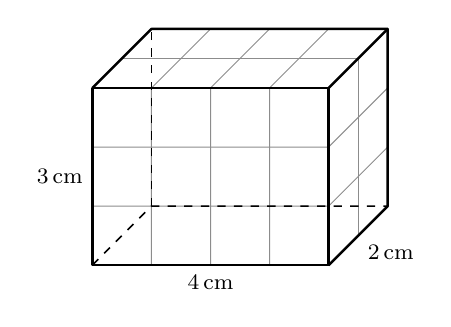
\begin{tikzpicture}[scale=0.75,font=\footnotesize,line join=round]\draw[black!45,line width=0.35pt] (1,0) -- (1,3) -- (2,4);\draw[black!45,line width=0.35pt] (2,0) -- (2,3) -- (3,4);\draw[black!45,line width=0.35pt] (3,0) -- (3,3) -- (4,4);\draw[black!45,line width=0.35pt] (0,1) -- (4,1) -- (5,2);\draw[black!45,line width=0.35pt] (0,2) -- (4,2) -- (5,3);\draw[black!45,line width=0.35pt] (0.5,3.5) -- (4.5,3.5) -- (4.5,0.5);\draw[line width=0.9pt] (0,0) rectangle (4,3);\draw[line width=0.9pt] (4,0) -- (5,1) -- (5,4) -- (1,4) -- (0,3);\draw[line width=0.9pt] (4,3) -- (5,4);\draw[dashed,line width=0.6pt] (0,0) -- (1,1) -- (5,1);\draw[dashed,line width=0.6pt] (1,1) -- (1,4);\node[below] at (2,0) {4\,cm};\node[left] at (0,1.5) {3\,cm};\node[below right] at (4.5,0.5) {2\,cm};\end{tikzpicture}}{}{}
\medskip
\aufg{\hangindent7mm\hangafter1\nr{2.}Berechne das Volumen eines Quaders mit $7$\,cm Länge, $4$\,cm Breite und $3$\,cm Höhe.}{}{}
\medskip
\aufg{\hangindent7mm\hangafter1\nr{3.}Ein Holzwürfel hat $6$\,cm Kantenlänge. Berechne sein Volumen.}{}{}
\medskip
\aufg{\hangindent7mm\hangafter1\nr{4.}Für den Umzug gibt es zwei Kisten. Die eine ist $6$\,dm lang, $4$\,dm breit und $3$\,dm hoch. Die andere ist ein Würfel mit $5$\,dm Kantenlänge. In welche Kiste passt mehr hinein, und um wie viel?}{}{{\scriptsize\color{mbgrau}Ziel\hspace{2mm}}}
\medskip
\par\vspace{3mm}\setlength{\kr}{\dimexpr\pagegoal-\pagetotal-10mm\relax}%
\ifdim\kr>12mm\karomerk{k}{A}\noindent{\scriptsize\color{mbgrau}Platz zum Rechnen}\par\nointerlineskip\vspace{1mm}\noindent
\begin{tikzpicture}\clip (0,0) rectangle ({\linewidth-0.5mm},\kr);\draw[black!16,line width=0.3pt,step=5mm] (0,0) grid (\linewidth,\kr);\end{tikzpicture}\fi\par
\clearpage\label{s:B}\noindent\colorbox{black!12}{\makebox[10mm]{\Large\bfseries\strut B}}\hspace{3mm}{\Large\bfseries Oberfläche}\par\smallskip
\noindent Die \textbf{Oberfläche} ist die ganze Hülle: alle sechs Rechtecke zusammen. Je zwei liegen sich gegenüber und sind gleich groß.\par\medskip
\noindent\textbf{Formel}\par\nopagebreak\noindent\hspace*{4mm}\begin{minipage}{\dimexpr\linewidth-4mm\relax}$O = 2 \cdot a \cdot b + 2 \cdot a \cdot c + 2 \cdot b \cdot c$ \qquad Würfel: $O = 6 \cdot a \cdot a$\end{minipage}\par\medskip
\noindent\textbf{Beispiel}\quad Eine Schachtel ist $6$\,cm lang, $4$\,cm breit und $3$\,cm hoch. Wie viel Pappe braucht man für sie? Wie viel ohne Deckel?\par\smallskip
\noindent\begin{minipage}[t]{0.6\linewidth}\vspace{0pt}\par\noindent\hangindent6mm\hangafter1\makebox[6mm][l]{\textbf{1}}Boden und Deckel: je $6 \cdot 4 = 24$\,cm².\par\smallskip\par\noindent\hangindent6mm\hangafter1\makebox[6mm][l]{\textbf{2}}Vorn und hinten: je $6 \cdot 3 = 18$\,cm².\par\smallskip\par\noindent\hangindent6mm\hangafter1\makebox[6mm][l]{\textbf{3}}Links und rechts: je $4 \cdot 3 = 12$\,cm².\par\smallskip\par\noindent\hangindent6mm\hangafter1\makebox[6mm][l]{\textbf{4}}Alle sechs zusammen: $O = 2 \cdot 24 + 2 \cdot 18 + 2 \cdot 12 = 108$\,cm². Flächen haben die Einheit cm².\par\smallskip\par\noindent\hangindent6mm\hangafter1\makebox[6mm][l]{\textbf{5}}Ohne Deckel fehlt ein Rechteck: $108 - 24 = 84$\,cm².\par\smallskip\par\noindent\hangindent6mm\hangafter1\makebox[6mm][l]{\textbf{6}}Beim Würfel sind alle sechs Flächen gleiche Quadrate: $O = 6 \cdot a \cdot a$.\par\smallskip\end{minipage}\hfill
\begin{minipage}[t]{0.37\linewidth}\vspace{0pt}\centering 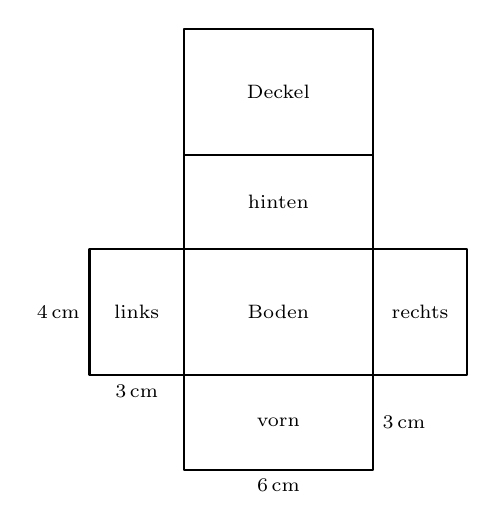
\begin{tikzpicture}[scale=0.4,font=\scriptsize,line join=round]\draw[line width=0.8pt] (3,0) rectangle (9,3);\node at (6.0,1.5) {vorn};\draw[line width=0.8pt] (3,3) rectangle (9,7);\node at (6.0,5.0) {Boden};\draw[line width=0.8pt] (3,7) rectangle (9,10);\node at (6.0,8.5) {hinten};\draw[line width=0.8pt] (3,10) rectangle (9,14);\node at (6.0,12.0) {Deckel};\draw[line width=0.8pt] (0,3) rectangle (3,7);\node at (1.5,5.0) {links};\draw[line width=0.8pt] (9,3) rectangle (12,7);\node at (10.5,5.0) {rechts};\node[below] at (6,0) {6\,cm};\node[right] at (9,1.5) {3\,cm};\node[left] at (0,5) {4\,cm};\node[below] at (1.5,3) {3\,cm};\end{tikzpicture}\end{minipage}\par\medskip
\noindent\textbf{Aufgaben}\hspace{1em}{\small\color{mbgrau}\karohinweis{B}{Rechne unten im Karo.}{Rechne auf einem extra Blatt.} Vergleiche jede Aufgabe gleich mit dem Lösungsheft.}\par\smallskip
\aufgg{\hangindent7mm\hangafter1\nr{1.}Berechne die Oberfläche des Quaders im Bild.}{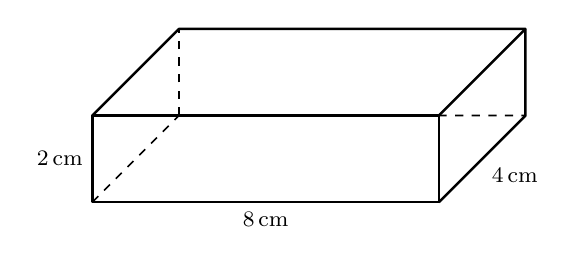
\begin{tikzpicture}[scale=0.55,font=\footnotesize,line join=round]\draw[line width=0.9pt] (0,0) rectangle (8,2);\draw[line width=0.9pt] (8,0) -- (10,2) -- (10,4) -- (2,4) -- (0,2);\draw[line width=0.9pt] (8,2) -- (10,4);\draw[dashed,line width=0.6pt] (0,0) -- (2,2) -- (10,2);\draw[dashed,line width=0.6pt] (2,2) -- (2,4);\node[below] at (4,0) {8\,cm};\node[left] at (0,1) {2\,cm};\node[below right] at (9,1) {4\,cm};\end{tikzpicture}}{}{}
\medskip
\aufg{\hangindent7mm\hangafter1\nr{2.}Ein Holzwürfel hat $10$\,cm Kantenlänge. Berechne seine Oberfläche.}{}{}
\medskip
\aufg{\hangindent7mm\hangafter1\nr{3.}Eine Kiste aus Holz hat keinen Deckel. Sie ist $5$\,dm lang, $4$\,dm breit und $2$\,dm hoch. Wie viele dm² Holz braucht man?}{}{}
\medskip
\aufg{\hangindent7mm\hangafter1\nr{4.}Tom baut ein Aquarium ohne Deckel aus Glas. Es soll $60$\,cm lang, $30$\,cm breit und $40$\,cm hoch werden. Er hat Glasplatten mit zusammen $8\,000$\,cm². Reicht das Glas? Begründe mit einer Rechnung.}{}{{\scriptsize\color{mbgrau}Ziel\hspace{2mm}}}
\medskip
\par\vspace{3mm}\setlength{\kr}{\dimexpr\pagegoal-\pagetotal-10mm\relax}%
\ifdim\kr>12mm\karomerk{k}{B}\noindent{\scriptsize\color{mbgrau}Platz zum Rechnen}\par\nointerlineskip\vspace{1mm}\noindent
\begin{tikzpicture}\clip (0,0) rectangle ({\linewidth-0.5mm},\kr);\draw[black!16,line width=0.3pt,step=5mm] (0,0) grid (\linewidth,\kr);\end{tikzpicture}\fi\par
\clearpage\label{s:C}\noindent\colorbox{black!12}{\makebox[10mm]{\Large\bfseries\strut C}}\hspace{3mm}{\Large\bfseries Liter und Kubikzentimeter}\par\smallskip
\noindent Ein Würfel mit $1$\,dm Kantenlänge fasst genau $1$ Liter. Weil $1$\,dm $= 10$\,cm ist, passen $10 \cdot 10 \cdot 10 = 1\,000$ Zentimeterwürfel hinein.\par\medskip
\noindent\textbf{Formel}\par\nopagebreak\noindent\hspace*{4mm}\begin{minipage}{\dimexpr\linewidth-4mm\relax}$1$ Liter $= 1$\,dm³ $= 1\,000$\,cm³ \qquad $1$\,m³ $= 1\,000$ Liter\end{minipage}\par\medskip
\noindent\textbf{Beispiel}\quad Ein Aquarium ist innen $40$\,cm lang, $25$\,cm breit und $30$\,cm hoch. Wie viele Liter Wasser passen hinein?\par\smallskip
\noindent\begin{minipage}[t]{0.6\linewidth}\vspace{0pt}\par\noindent\hangindent6mm\hangafter1\makebox[6mm][l]{\textbf{1}}Volumen in cm³: $V = 40 \cdot 25 \cdot 30 = 30\,000$\,cm³.\par\smallskip\par\noindent\hangindent6mm\hangafter1\makebox[6mm][l]{\textbf{2}}$1\,000$\,cm³ sind $1$ Liter. Also durch $1\,000$ teilen: $30\,000 : 1\,000 = 30$, das sind $30$ Liter.\par\smallskip\par\noindent\hangindent6mm\hangafter1\makebox[6mm][l]{\textbf{3}}Rückwärts mal $1\,000$: $2$ Liter $= 2\,000$\,cm³. Ein dm³ ist genau ein Liter: $2$\,dm³ $= 2$ Liter.\par\smallskip\par\noindent\hangindent6mm\hangafter1\makebox[6mm][l]{\textbf{4}}Große Becken misst man in m: $1$\,m³ $= 1\,000$ Liter, also $3$\,m³ $= 3\,000$ Liter.\par\smallskip\end{minipage}\hfill
\begin{minipage}[t]{0.37\linewidth}\vspace{0pt}\centering 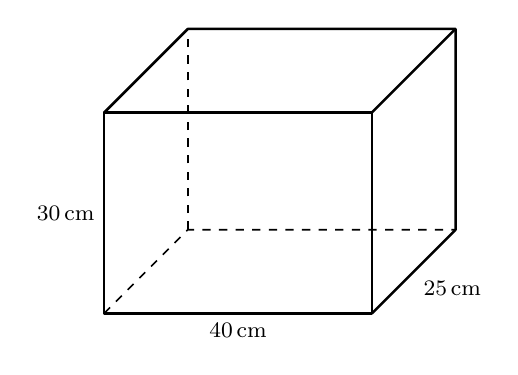
\begin{tikzpicture}[scale=0.85,font=\footnotesize,line join=round]\draw[line width=0.9pt] (0,0) rectangle (4,3);\draw[line width=0.9pt] (4,0) -- (5.25,1.25) -- (5.25,4.25) -- (1.25,4.25) -- (0,3);\draw[line width=0.9pt] (4,3) -- (5.25,4.25);\draw[dashed,line width=0.6pt] (0,0) -- (1.25,1.25) -- (5.25,1.25);\draw[dashed,line width=0.6pt] (1.25,1.25) -- (1.25,4.25);\node[below] at (2,0) {40\,cm};\node[left] at (0,1.5) {30\,cm};\node[below right] at (4.625,0.625) {25\,cm};\end{tikzpicture}\end{minipage}\par\medskip
\noindent\textbf{Aufgaben}\hspace{1em}{\small\color{mbgrau}\karohinweis{C}{Rechne unten im Karo.}{Rechne auf einem extra Blatt.} Vergleiche jede Aufgabe gleich mit dem Lösungsheft.}\par\smallskip
\aufg{\hangindent7mm\hangafter1\nr{1.}Rechne um: $5\,000$\,cm³ in Liter; \quad $3$ Liter in cm³; \quad $2\,500$\,cm³ in Liter; \quad $4$\,m³ in Liter.}{}{}
\medskip
\aufg{\hangindent7mm\hangafter1\nr{2.}Ein Karton ist innen $30$\,cm lang, $20$\,cm breit und $10$\,cm hoch. Wie viele Liter passen hinein?}{}{}
\medskip
\aufg{\hangindent7mm\hangafter1\nr{3.}Ein Wasserbecken im Garten ist ein Quader: $3$\,m lang, $2$\,m breit und $1$\,m tief. Wie viele Liter Wasser passen hinein?}{}{}
\medskip
\aufg{\hangindent7mm\hangafter1\nr{4.}Im Prospekt steht über ein Aquarium: „innen $60$\,cm lang, $30$\,cm breit, $35$\,cm hoch, fasst $72$ Liter“. Stimmt die Angabe?\par\smallskip\leftskip7mm \kreuz{Ja, es passen $72$ Liter hinein.}\ \kreuz{Nein, es passt weniger hinein.}\par\kreuz{Nein, es passt mehr hinein.}}{}{{\scriptsize\color{mbgrau}Ziel\hspace{2mm}}}
\medskip
\par\vspace{3mm}\setlength{\kr}{\dimexpr\pagegoal-\pagetotal-10mm\relax}%
\ifdim\kr>12mm\karomerk{k}{C}\noindent{\scriptsize\color{mbgrau}Platz zum Rechnen}\par\nointerlineskip\vspace{1mm}\noindent
\begin{tikzpicture}\clip (0,0) rectangle ({\linewidth-0.5mm},\kr);\draw[black!16,line width=0.3pt,step=5mm] (0,0) grid (\linewidth,\kr);\end{tikzpicture}\fi\par
\clearpage\label{s:D}\noindent\colorbox{black!12}{\makebox[10mm]{\Large\bfseries\strut D}}\hspace{3mm}{\Large\bfseries Höhe aus dem Volumen}\par\smallskip
\noindent Kennst du das Volumen, die Länge und die Breite, rechnest du rückwärts: Volumen geteilt durch die Grundfläche (Länge mal Breite) gibt die Höhe.\par\medskip
\noindent\textbf{Formel}\par\nopagebreak\noindent\hspace*{4mm}\begin{minipage}{\dimexpr\linewidth-4mm\relax}$c = V : (a \cdot b)$\end{minipage}\par\medskip
\noindent\textbf{Beispiel}\quad In ein Aquarium (innen $50$\,cm lang, $30$\,cm breit, $40$\,cm hoch) werden $45$ Liter Wasser gefüllt. Wie hoch steht das Wasser? Wie viel bleibt bis zum Rand frei?\par\smallskip
\noindent\begin{minipage}[t]{0.6\linewidth}\vspace{0pt}\par\noindent\hangindent6mm\hangafter1\makebox[6mm][l]{\textbf{1}}Liter in cm³: $45$ Liter $= 45\,000$\,cm³.\par\smallskip\par\noindent\hangindent6mm\hangafter1\makebox[6mm][l]{\textbf{2}}Grundfläche: Länge mal Breite, $50 \cdot 30 = 1\,500$\,cm².\par\smallskip\par\noindent\hangindent6mm\hangafter1\makebox[6mm][l]{\textbf{3}}Höhe: Volumen durch Grundfläche, $45\,000 : 1\,500 = 30$\,cm.\par\smallskip\par\noindent\hangindent6mm\hangafter1\makebox[6mm][l]{\textbf{4}}Probe: $50 \cdot 30 \cdot 30 = 45\,000$\,cm³. Stimmt.\par\smallskip\par\noindent\hangindent6mm\hangafter1\makebox[6mm][l]{\textbf{5}}Bis zum Rand: $40 - 30 = 10$\,cm frei.\par\smallskip\end{minipage}\hfill
\begin{minipage}[t]{0.37\linewidth}\vspace{0pt}\centering 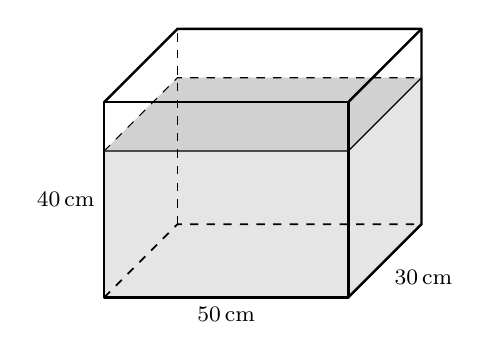
\begin{tikzpicture}[scale=0.62,font=\footnotesize,line join=round]\fill[black!10] (0,0) -- (5,0) -- (6.5,1.5) -- (6.5,4.5) -- (1.5,4.5) -- (0,3) -- cycle;\fill[black!18] (0,3) -- (5,3) -- (6.5,4.5) -- (1.5,4.5) -- cycle;\draw[line width=0.5pt] (0,3) -- (5,3) -- (6.5,4.5);\draw[dashed,line width=0.4pt] (0,3) -- (1.5,4.5) -- (6.5,4.5);\draw[line width=0.9pt] (0,0) rectangle (5,4);\draw[line width=0.9pt] (5,0) -- (6.5,1.5) -- (6.5,5.5) -- (1.5,5.5) -- (0,4);\draw[line width=0.9pt] (5,4) -- (6.5,5.5);\draw[dashed,line width=0.6pt] (0,0) -- (1.5,1.5) -- (6.5,1.5);\draw[dashed,line width=0.6pt] (1.5,1.5) -- (1.5,5.5);\node[below] at (2.5,0) {50\,cm};\node[left] at (0,2) {40\,cm};\node[below right] at (5.75,0.75) {30\,cm};\end{tikzpicture}\end{minipage}\par\medskip
\noindent\textbf{Aufgaben}\hspace{1em}{\small\color{mbgrau}\karohinweis{D}{Rechne unten im Karo.}{Rechne auf einem extra Blatt.} Vergleiche jede Aufgabe gleich mit dem Lösungsheft.}\par\smallskip
\aufg{\hangindent7mm\hangafter1\nr{1.}Ein Quader hat das Volumen $60$\,cm³. Er ist $5$\,cm lang und $4$\,cm breit. Wie hoch ist er?}{}{}
\medskip
\aufg{\hangindent7mm\hangafter1\nr{2.}Ein Karton fasst $12$ Liter. Er ist innen $30$\,cm lang und $20$\,cm breit. Wie hoch ist er innen?}{}{}
\medskip
\aufg{\hangindent7mm\hangafter1\nr{3.}Ein Aquarium ist innen $60$\,cm lang und $25$\,cm breit. Es werden $30$ Liter Wasser eingefüllt. Wie hoch steht das Wasser?}{}{}
\medskip
\aufg{\hangindent7mm\hangafter1\nr{4.}Max füllt $98$ Liter Wasser in sein Aquarium. Es ist innen $70$\,cm lang, $40$\,cm breit und $45$\,cm hoch. Seine Fische springen gern, darum sollen bis zum Rand mindestens $8$\,cm frei bleiben. Ist das so?}{}{{\scriptsize\color{mbgrau}Ziel\hspace{2mm}}}
\medskip
\par\vspace{3mm}\setlength{\kr}{\dimexpr\pagegoal-\pagetotal-10mm\relax}%
\ifdim\kr>12mm\karomerk{k}{D}\noindent{\scriptsize\color{mbgrau}Platz zum Rechnen}\par\nointerlineskip\vspace{1mm}\noindent
\begin{tikzpicture}\clip (0,0) rectangle ({\linewidth-0.5mm},\kr);\draw[black!16,line width=0.3pt,step=5mm] (0,0) grid (\linewidth,\kr);\end{tikzpicture}\fi\par
\clearpage\label{s:T}\noindent\colorbox{black!12}{\makebox[10mm]{\Large\bfseries\strut T}}\hspace{3mm}{\Large\bfseries Probetest}\par\smallskip
\noindent Gemischt wie in der Prüfung, ohne Beispiel. Etwa 20 Minuten.\par\medskip
\noindent\textbf{Aufgaben}\hspace{1em}{\small\color{mbgrau}\karohinweis{T}{Rechne unten im Karo.}{Rechne auf einem extra Blatt.} Vergleiche jede Aufgabe gleich mit dem Lösungsheft.}\par\smallskip
\aufg{\hangindent7mm\hangafter1\nr{1.}Ein Würfel hat die Kantenlänge $4$\,cm. Wie groß ist sein Volumen?\par\smallskip\leftskip7mm \kreuz{$16$\,cm³}\ \kreuz{$48$\,cm³}\par\kreuz{$64$\,cm³}\ \kreuz{$96$\,cm³}}{}{}
\medskip
\aufg{\hangindent7mm\hangafter1\nr{2.}Wie viele Liter sind $6\,500$\,cm³?}{}{}
\medskip
\aufg{\hangindent7mm\hangafter1\nr{3.}Ein Quader ist $6$\,cm lang, $5$\,cm breit und $3$\,cm hoch. Berechne sein Volumen und seine Oberfläche.}{}{}
\medskip
\aufg{\hangindent7mm\hangafter1\nr{4.}Eine Schachtel fasst $2$ Liter. Sie ist innen $20$\,cm lang und $10$\,cm breit. Wie hoch ist sie innen?}{}{}
\medskip
\aufg{\hangindent7mm\hangafter1\nr{5.}Ein Aquarium ist innen $80$\,cm lang, $30$\,cm breit und $50$\,cm hoch. Es soll bis $10$\,cm unter den Rand gefüllt werden. Reichen $100$ Liter Wasser?}{}{{\scriptsize\color{mbgrau}Ziel\hspace{2mm}}}
\medskip
\par\vspace{3mm}\setlength{\kr}{\dimexpr\pagegoal-\pagetotal-10mm\relax}%
\ifdim\kr>12mm\karomerk{k}{T}\noindent{\scriptsize\color{mbgrau}Platz zum Rechnen}\par\nointerlineskip\vspace{1mm}\noindent
\begin{tikzpicture}\clip (0,0) rectangle ({\linewidth-0.5mm},\kr);\draw[black!16,line width=0.3pt,step=5mm] (0,0) grid (\linewidth,\kr);\end{tikzpicture}\fi\par
\end{document}
